\documentclass[11pt]{article}
\usepackage{geometry}
\geometry{a4paper, portrait, margin=2.5cm}
\usepackage{graphicx}
\bibliographystyle{abbrv}

\title{Determining the Height of the Rayleigh-Taylor Instability}
\author{J.T.Horne}

\begin{document}
\maketitle	

\section*{Introduction}

The Rayleigh-Taylor instability is an instability seen at an interface between two fluids of different densities. It occurs when the light fluid is pushing the heavy fluid. The simplest example, and the experimental set up used here, is a denser fluid located above a lighter fluid with a flat interface between them. Assuming that there is an initial perturbation, which will be the case in any real world scenario, the instability will grow with a finger-like pattern until it breaks down into a turbulent mixing flow \cite{sharp1984RToverview}. This report will consider the various different criteria for determining the height of the instability.

\section*{Theory}

\subsection*{Instability Growth}

Basic theory

\subsection*{Instability Height Criteria}

Various height criteria

\section*{Simulation}

The first approach taken for assessing the instability height criteria was to use them to track the development of an 'ideal' 2D Rayleigh-Taylor case. This ideal case was produced using the MOBILE incompressible flow solver.

\subsection*{MOBILE Incompressible Flow Solver}

Brief summary of workings of MOBILE

\subsection*{Results}

MOBILE produces a sequence of images showing the progression of the flow through time. These are treated as frames in a video, as is output from the experiments. In this way the simulation data was processed in an identical manner as the experimental data and gave a fair assessment of the performance of the instability height criteria for both simulation and experiments.

\section*{Experiments}

A more rigorous test of the criteria, and of their implementation, is how well they perform on experimental data.

\subsection*{Methodology}

A two fluid system of fresh water and salt water was set up in a thin tank to produce a flow akin to a 2D case. The tank was constructed from two acrylic sheets with a gasket clamped between them. Valved bulkheads were installed in diagonally opposing corners of the tank to allow the supply of the two fluids. The depth of the tank can be increased by the addition of a spacer plate between the two walls, but this was not used during these experiments and hence the dimensions of the working volume were w mm x h mm x d mm.

The experiment requires the means by which to create the initial conditions of a denser fluid above a lighter fluid, instigate the instability growth from a defined start point and record the development of the instability. The initialisation of an unstable system was achieved by mounting the tank in a set of frames on gimbals to allow rotation in all 3 axes (although only one axis of rotation was required in the experiment itself), as seen in figure \ref{fig:gimbalframes1}. This allowed for the tank to be filled with a stable system of salt water below fresh water, with a well defined interface between the liquids. The tank was then flipped about the horizontal axis parallel to the interface to invert the system into the unstable configuration of salt water above fresh water.

\begin{figure}
\centering
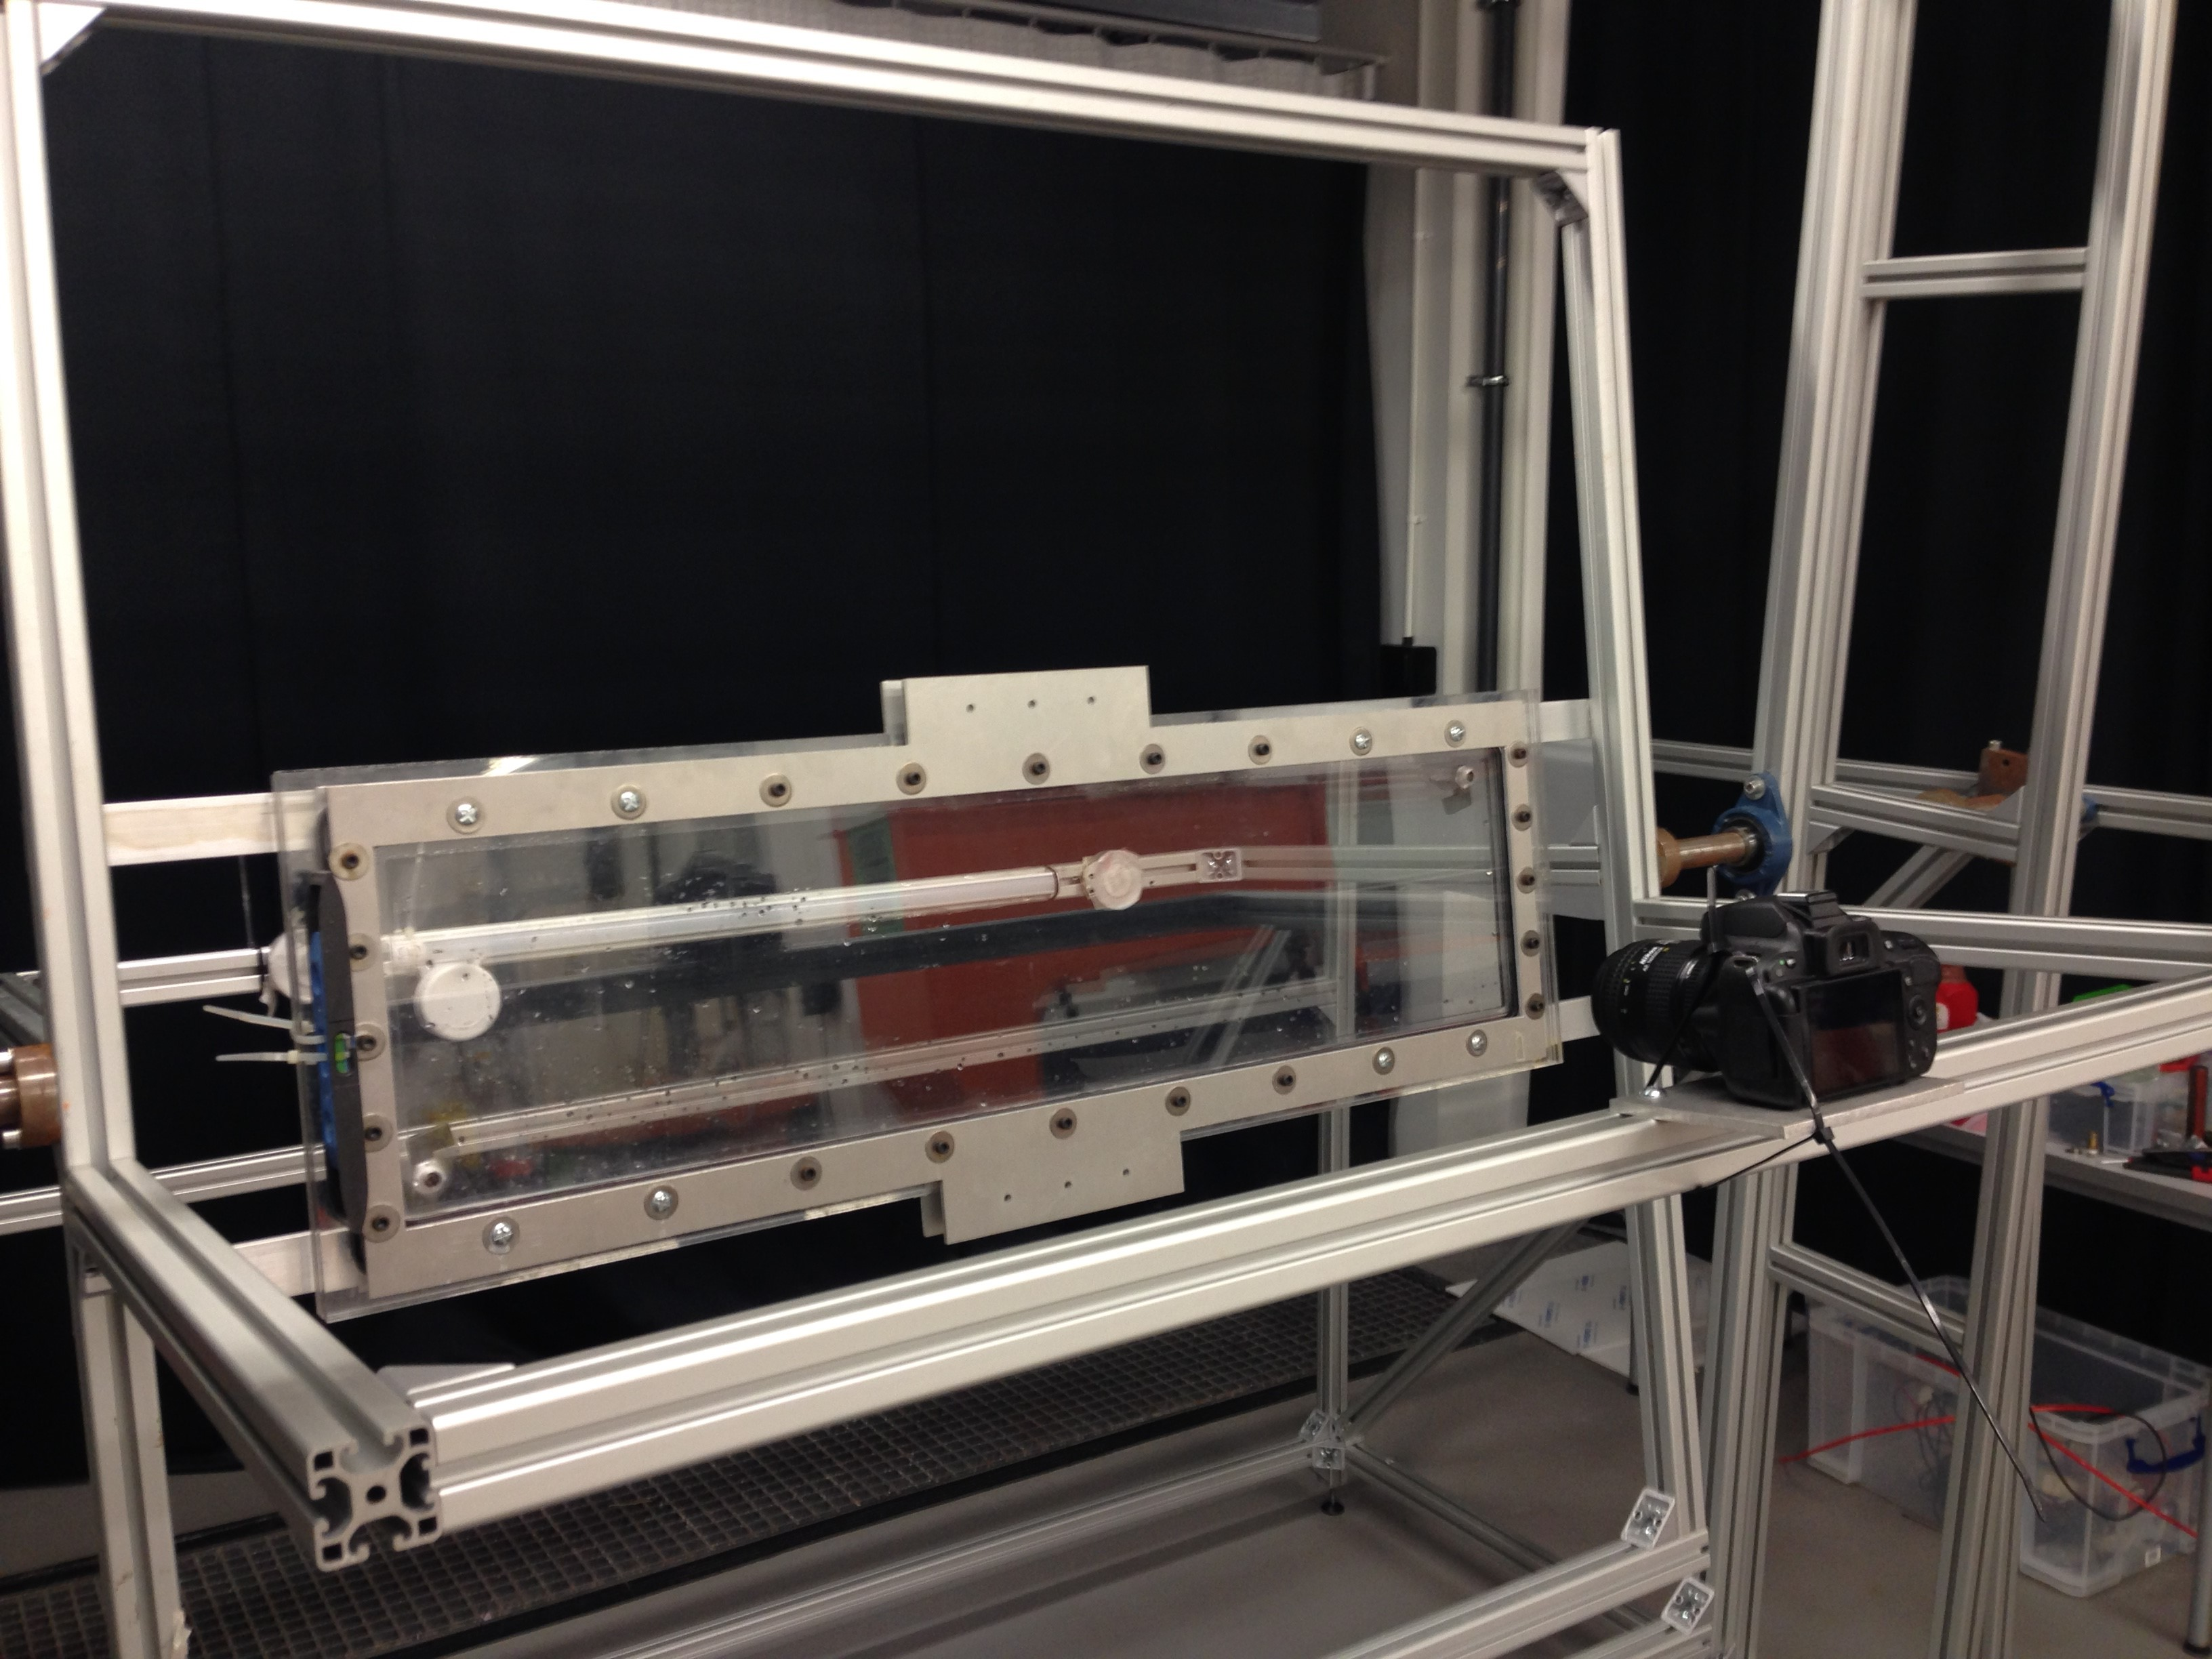
\includegraphics[width=0.8\textwidth]{gimbal_frame}
\caption{Two dimensional tank mounted on frames on gimbals to allow for rotation of the tank}
\label{fig:gimbalframes1}	
\end{figure}

The salt water was dyed using red food colouring to visually distinguish between the two liquids. The colour of the liquid in any mixing therefore indicates the density of the resulting fluid. The experiment was recorded using a video camera mounted in a fixed position relative to the tank (i.e. rotating with the tank), which allowed for direct use of the video to calculate the height of the instability without having to account for the changing position of the tank or parallax due to the camera location. The quality and repeatability of the images of the fluid was improved by installing a strip light directly opposite to the camera with respect to the tank and also fixed relative to the tank. A layer of tracing paper was fixed to the light-side of the tank, giving suitably diffuse light. The experiments were conducted in low level ambient light to avoid issues with glare or reflections, which could give errors in the results.
	
\subsection*{Results}



\section*{Conclusion}



\bibliography{../../Literature/References}

\end{document}          
